\documentclass[runningheads]{llncs}

\usepackage[T1]{fontenc}
\usepackage[utf8]{inputenc}
\usepackage{graphicx}
\usepackage{booktabs}
\usepackage{amsmath}
\usepackage{amssymb}
\usepackage{xurl}          % lets long URLs break instead of running off the margin
\usepackage{tikz}
\usetikzlibrary{arrows.meta,positioning}

% Absorbs the last few points of overfull lines without visibly loosening spacing.
\setlength{\emergencystretch}{3em}

% Springer's own abstract style insets the block 1 cm on both sides and runs the
% word "Abstract." into the first line as a side label. Set the block flush with
% the text width and give the heading its own line. Revert by deleting this block
% if the target venue enforces the stock layout.
\makeatletter
\def\abstractname{Abstract}
\renewenvironment{abstract}{%
  \list{}{\advance\topsep by0.35cm\relax\small
    \leftmargin=\z@
    \rightmargin=\z@
    \labelwidth=\z@
    \listparindent=\z@
    \itemindent=\z@}%
  \item[]{\centering\bfseries\abstractname\par}\nobreak\vskip 3pt\noindent\ignorespaces}%
  {\endlist}
\makeatother

\begin{document}

\title{When Graph-Derived Neighbourhood Features Do Not Help:
A Leakage-Controlled Evaluation of Behavioural-LRFM Churn Prediction
in Non-Contractual Retail}

\titlerunning{When Graph-Derived Neighbourhood Features Do Not Help}

% Affiliation first, then names, then e-mails (author's requested order).
\author{{\small FPT University, Ho Chi Minh City, Vietnam}\\[4pt]
Duc Nhat Vo\textsuperscript{a}, Gia Bao Duong\textsuperscript{b},
Nguyen Minh Hai Tran\textsuperscript{c}}
\authorrunning{D. N. Vo et al.}
\institute{\email{\textsuperscript{a}voducnhat242006@gmail.com,
\textsuperscript{b}ilyrabao@gmail.com,
\textsuperscript{c}trannguyenminhhai265@gmail.com}}

\maketitle

\begin{abstract}
Customer similarity graphs are an appealing addition to RFM-style churn models.
If churn spreads through behavioural peer groups, the churn rate among a
customer's nearest neighbours should help predict that customer's own churn. We
test that idea on the Online Retail II dataset under two controls. First, the
neighbourhood and community churn rates are recomputed inside every training
fold, so no test label reaches the feature matrix. Second, every comparison runs
over ten repetitions of five-fold cross-validation and is judged by the corrected
resampled $t$-test rather than by a single split. Under these controls the idea
does not hold. With the classifier fixed, no feature tier beats a plain
three-variable RFM baseline, on either ROC-AUC or PR-AUC, for either classifier,
at any graph degree from 5 to 20. The graph-enhanced tier gains $+0.0033$ ROC-AUC
on one fold partition and reverses sign across ten. Every significant difference
involves a change of classifier, so none speaks to the graph features. Attribution and contribution also come apart: the
neighbourhood churn rate ranks third by SHAP, yet removing the graph features
costs nothing. Because the $k$-NN graph is built on the features the classifier
already uses, its neighbourhood churn rate largely restates existing information
by construction; a graph built from co-purchase or referral links may behave
differently. We argue that single-split evaluation cannot separate an effect this
small from fold noise.

\keywords{Churn prediction \and RFM \and Customer similarity graph \and
Community detection \and Repeated cross-validation \and Negative result.}
\end{abstract}

\section{Introduction}

Non-contractual retail gives no cancellation signal. A customer who stops buying
does not announce it, so churn has to be defined by inactivity over a chosen
horizon, and the modelling task is to predict that inactivity from purchase
history. The RFM representation (recency, frequency, monetary value) has been
the working vocabulary of this problem for decades, and a large applied
literature extends it: adding relationship length, adding demographic attributes
\cite{ho2023extended}, or unrolling the triple over time
\cite{mena2023timevarying}.

A more recent line treats the customer base as a graph rather than a table.
Corr\^{e}a Vianna Filho et al.\ formulate RFM segmentation as a maximum $k$-cut
problem on a customer graph, where identical score vectors collapse into
super-vertices and the reduced graph is bounded independently of the number of
customers \cite{viannafilho2026rfm}. Once customers are vertices, a next step
suggests itself: if a similarity graph can be built, then community detection
\cite{blondel2008louvain,traag2019leiden} can partition it, and graph-derived
quantities such as degree, centrality and, in particular, the churn rate observed
among a customer's neighbours can be appended to the feature matrix of a supervised
churn model. The underlying hypothesis is a contagion one: churn risk is partly a
property of the behavioural neighbourhood, not only of the individual.

This paper tests that hypothesis and does not find support for it. We build the
pipeline the hypothesis calls for: a nine-dimensional behavioural extension of
RFM, a $k$-nearest-neighbour customer similarity graph, Louvain and Leiden
communities, and graph node features including neighbour and community churn
rates. We then evaluate it against progressively simpler feature sets. The
evaluation is where the contribution lies. Two controls turn out to be decisive:

\begin{enumerate}
\item \textbf{Fold-local recomputation of the neighbourhood features.} Both are
aggregates of the target, so computing them once over the full dataset places
test labels inside the training features. We recompute them inside every training
fold from training labels only.
\item \textbf{Repeated cross-validation with a variance-corrected test.} A single
split gives a point estimate with no uncertainty attached. We use ten repetitions
on a shared fold partition and report the corrected resampled $t$-test of Nadeau
and Bengio \cite{nadeau2003inference}, which adjusts for the training-set overlap
that makes the naive paired test anti-conservative
\cite{dietterich1998approximate,bouckaert2004replicability}.
\end{enumerate}

With both controls in place, the effect the pipeline was built to demonstrate
disappears. We state our contributions conservatively:

\begin{itemize}
\item A negative result, reported as such: with the classifier fixed, neither
the behavioural extension nor the graph features improve discrimination over a
three-variable RFM baseline, at any graph degree tested.
\item An evaluation protocol for this application area, together with the
observation that differences below roughly $0.005$ ROC-AUC on this dataset are
distinguishable neither from fold noise nor from library-version drift.
\item A dissociation between SHAP attribution rank and predictive contribution,
which we state explicitly because feature-importance rankings are frequently read
as evidence of usefulness.
\end{itemize}

\section{Related Work}

Three strands meet in this problem, and the tension between them is what makes a
negative result informative rather than merely disappointing.

The \emph{representation} strand asks what to measure about a customer. RFM
persists because it is cheap and interpretable, and the extensions that follow it
generally add dimensions rather than replace the idea: relationship length
alongside the original three, demographic attributes \cite{ho2023extended}, or a
temporal unrolling in which the RFM triple becomes a sequence rather than a point
\cite{mena2023timevarying}. What these extensions share is an implicit claim that
the added dimensions carry information the original three do not. That claim is
testable, and it is one of the things we test.

The \emph{structural} strand asks whether customers should be modelled jointly
rather than independently. Vianna Filho et al.\ make the strongest form of this
argument for segmentation: by recasting RFM segmentation as maximum $k$-cut over
a customer graph, the segmentation objective becomes an explicit graph quantity
rather than a by-product of a distance-based clustering heuristic
\cite{viannafilho2026rfm}. Their work is the starting point of ours, but it stops
at segmentation and does not address supervised prediction. Community detection
supplies the machinery for a supervised extension: modularity-based partitioning
\cite{newman2004community,blondel2008louvain} and its refinement guaranteeing
well-connected communities \cite{traag2019leiden} are standard, well-implemented,
and apply directly to a similarity graph over customers. The step from there to
appending the neighbourhood churn rate as a feature is short, which is precisely
why it deserves scrutiny: that feature is an aggregate of the label, and features
of this kind are the classic vehicle for target leakage.

The neighbourhood-churn feature is not itself new, and the settings where it has
worked are informative. Telecommunications studies build it from call-detail
records, where an edge means two subscribers actually spoke, and report that a
subscriber's risk rises with the number of churned neighbours
\cite{kostic2020socialnetwork}; more recent work treats the social graph as a
temporal object and predicts churn from how it evolves
\cite{lee2025tempodegraphnet}. What separates those settings from ours is what an
edge means. Theirs records an interaction that exists independently of the
model's feature matrix; ours records proximity within the very feature space the
classifier already sees. That difference turns out to matter, and
Sect.~\ref{sec:contagion} returns to it.

The \emph{evaluation} strand is where the applied literature is weakest and where
the methodological literature has long been settled. Overlapping resampled
training sets inflate Type I error in the tests normally used to compare learning
algorithms \cite{dietterich1998approximate}; the variance correction that repairs
the paired test for exactly this case has been available for two decades
\cite{nadeau2003inference}, along with evidence on how such tests replicate in
practice \cite{bouckaert2004replicability,demsar2006statistical}. Applied churn
studies, including our own earlier reporting of the present pipeline,
nonetheless rank configurations by a single cross-validated point estimate. At
differences on the order of $10^{-3}$ ROC-AUC that cannot separate an effect from
a fold partition. Our results are an instance of the gap between these two
strands, not a criticism of any individual study.

Gradient-boosted trees \cite{chen2016xgboost,ke2017lightgbm} and additive feature
attribution \cite{lundberg2017shap} are used here as standard tools, not as
objects of study.

\section{Pipeline Overview}

Figure~\ref{fig:pipeline} shows the stages. The upper row builds the
representation; the lower row, read right to left, carries it through the two
controls into the evaluation.

\begin{figure}[t]
\centering
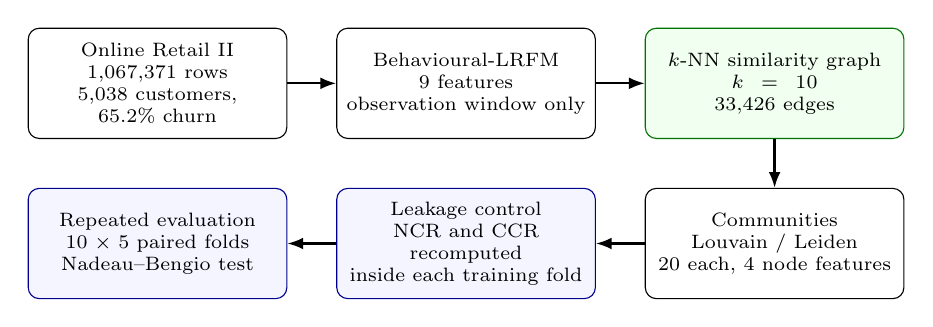
\begin{tikzpicture}[
  node distance=0.62cm and 0.62cm,
  flowbox/.style={draw, rounded corners, align=center, text width=3.05cm,
                  minimum height=1.4cm, font=\scriptsize},
  focusbox/.style={flowbox, draw=green!45!black, fill=green!6},
  ctrlbox/.style={flowbox, draw=blue!55!black, fill=blue!4},
  arrow/.style={-{Latex[length=2.0mm]}, thick}
]
\node[flowbox] (data) {Online Retail II\\1{,}067{,}371 rows\\5{,}038 customers, 65.2\% churn};
\node[flowbox, right=of data] (feat) {Behavioural-LRFM\\9 features\\observation window only};
\node[focusbox, right=of feat] (graph) {$k$-NN similarity graph\\$k=10$\\33{,}426 edges};
\node[flowbox, below=of graph] (comm) {Communities\\Louvain / Leiden\\20 each, 4 node features};
\node[ctrlbox, below=of feat] (leak) {Leakage control\\NCR and CCR recomputed\\inside each training fold};
\node[ctrlbox, below=of data] (eval) {Repeated evaluation\\$10 \times 5$ paired folds\\Nadeau--Bengio test};
\draw[arrow] (data.east) -- (feat.west);
\draw[arrow] (feat.east) -- (graph.west);
\draw[arrow] (graph.south) -- (comm.north);
\draw[arrow] (comm.west) -- (leak.east);
\draw[arrow] (leak.west) -- (eval.east);
\end{tikzpicture}
\caption{Analysis pipeline. Green: the component under test. Blue: the two
controls that determine the result, fold-local recomputation of the
label-derived features and repeated evaluation with a variance-corrected test.}
\label{fig:pipeline}
\end{figure}

\section{Data and Feature Construction}

\subsection{Dataset and Windows}

We use Online Retail II, the transaction log of a UK-based non-store retailer
covering December 2009 to December 2011, distributed through the UCI Machine
Learning Repository \cite{uci2019onlineretail} and introduced in the RFM
segmentation study of Chen et al.\ \cite{chen2012datamining}. The raw file
contains $1{,}067{,}371$ transaction rows
across two worksheets ($525{,}461$ and $541{,}910$); the $541{,}000$ figure often
quoted for this dataset is the second worksheet alone.

Features and labels are separated in time. The observation window covers
transactions from 2009-12-01 up to the timestamp 2011-06-30 00:00 and is the
only period from which features are computed. The prediction window covers the
following three months, up to 2011-09-30 00:00 (92 days); a customer active in
the observation window is labelled a churner if no purchase appears in the
prediction window. After filtering to valid transactions inside the observation
window ($556{,}212$ rows) and aggregating to the customer level, the working
matrix contains $5{,}038$ customers. The churn rate is $65.2\%$.

That last number deserves emphasis, because it inverts an assumption often
carried into this problem. Churners are the \emph{majority} class here, not a
rare positive to be rescued by resampling. A three-month inactivity horizon
applied to a retailer with long interpurchase intervals labels most of the base
as churned.
This makes PR-AUC less informative than it would be under genuine imbalance, and
we report it alongside ROC-AUC rather than as the primary metric.

\subsection{Behavioural-LRFM Features}

Nine customer-level features are computed inside the observation window: length
$L$ (days from the first purchase to the analysis date 2011-07-01), recency $R$
(days from the last purchase to the same date), frequency $F$ (distinct
invoices), monetary value $M$, average order value, basket size, product
diversity, cancellation rate, and mean interpurchase time. Cancellation rate is
restricted to cancellations dated inside the observation window; an earlier
version of this pipeline computed it over the full log, which allowed
post-window cancellations to enter a pre-window feature.

\section{Graph Construction and Community Detection}

The nine features are standardised and a $k$-nearest-neighbour graph is built
over customers with $k = 10$ and Euclidean distance, with edge weight
$w(i,j) = 1/(1 + d(i,j))$. The resulting graph has $5{,}038$ nodes and $33{,}426$
edges. Louvain \cite{blondel2008louvain} yields 20 communities with modularity
$0.8385$; Leiden \cite{traag2019leiden} yields 20 communities with modularity
$0.8323$.

The high modularity should not be over-read: a $k$-NN graph with fixed $k$ imposes
near-uniform degree and strong local clustering by construction, so a value above
$0.8$ reflects how the graph was built at least as much as any structure in the
customer base.

Six graph-derived features are appended: degree, weighted degree, PageRank,
clustering coefficient, and the two neighbourhood aggregates that motivate the
design: neighbour churn rate (mean label among a customer's own $k$ nearest
neighbours) and community churn rate (mean label within the customer's Louvain
community).

\section{Leakage Controls}

Both neighbourhood aggregates are functions of the target. Computing either over
the full dataset before cross-validation lets the label of a test customer
influence the training features of its neighbours, and the resulting optimism can
be substantial. We therefore recompute both inside each training fold: for
customer $i$, the neighbour churn rate averages labels over
$\mathcal{N}(i) \cap \mathcal{T}$, where $\mathcal{N}(i)$ is the set of the $k$
nearest neighbours of $i$ and $\mathcal{T}$ is the training index set,
falling back to the training-fold base rate when that intersection is empty; the
community churn rate is computed the same way within each Louvain community. The
graph and the communities themselves are built from features only, never from
labels, and are therefore fixed across folds.

Three further controls apply throughout. The classifier's scaler is fitted inside
each training fold; the graph, its scaling and the K-means segments use all
customers' features but no labels. K-means and Louvain cluster identifiers are
one-hot encoded rather than passed as integers. Louvain and Leiden are both
reported, but the repeated-CV features use Louvain.

\section{Evaluation Protocol}

\subsection{Feature Tiers}

Five nested tiers isolate the contribution of each modelling layer:
\textbf{RFM} ($R, F, M$); \textbf{LRFM} (adding $L$); \textbf{B-LRFM} (the nine
behavioural features); \textbf{B-LRFM+Seg} (adding 23 one-hot segment and
community indicators); and \textbf{Graph-Enhanced}, the full 38-feature matrix
adding the four static graph features and the two fold-local neighbourhood
aggregates. Two classifiers are evaluated on every tier: LightGBM
\cite{ke2017lightgbm} as the primary model and $\ell_2$-regularised logistic
regression as an interpretable reference.

\subsection{Repeated Cross-Validation and Significance}
\label{sec:sig}

We run ten repetitions of stratified five-fold cross-validation, giving 50 folds.
Within a repetition all five tiers and both classifiers see the \emph{same} fold
partition, so per-fold differences are properly paired. For a difference
$d_1, \dots, d_n$ over $n = 50$ folds we report the corrected resampled
$t$-statistic \cite{nadeau2003inference}
\begin{equation}
t = \frac{\bar{d}}
{\sqrt{\hat{\sigma}^{2}\left(\dfrac{1}{n} + \dfrac{n_{2}}{n_{1}}\right)}},
\qquad \frac{n_{2}}{n_{1}} = \frac{1}{4},
\end{equation}
where $n_{2}/n_{1}$ is the ratio of test-set to training-set size, which for
five-fold cross-validation is $1/4$. We report $p_{\mathrm{NB}}$ from this
statistic only. Bootstrap confidence intervals over the 50 differences are given
for effect magnitude, but we caution against reading them as significance
statements: the bootstrap resamples the differences as if independent, while
repeated folds share training data, so those intervals are narrower than the
correlation structure warrants. This is the same overlap that makes the naive
paired $t$-test anti-conservative \cite{dietterich1998approximate}.

Run with the single seed used by the original pipeline, the significance harness
reproduces that pipeline's per-tier ROC-AUC to four decimal places on all five
tiers, so any divergence below is attributable to the fold partition rather than
to a re-implementation difference.

\section{Results}
\label{sec:results}

\subsection{One Split Says the Opposite of Ten}
\label{sec:onesplit}

Table~\ref{tab:main} puts the two evaluations side by side, and the contrast is
the result of this paper. On the single stratified five-fold split this pipeline
originally reported, Graph-Enhanced is the best tier, $+0.0033$ ROC-AUC above
RFM. Over ten repetitions it is jointly the worst, $-0.0021$ below RFM. Nothing
about the model changed between those two columns; only the fold partition did. Even at the
seed that produces it, the $+0.0033$ gap has a bootstrap 95\% interval of
$[-0.0025, +0.0099]$, which contains zero.

\begin{table}[t]
\centering
\caption{LightGBM across the five feature tiers. The single-split column is the
seed-42 evaluation this pipeline first reported; the remaining columns are ten
repetitions of the same protocol. $p_{\mathrm{NB}}$ is the corrected resampled
$t$-test against RFM (Sect.~\ref{sec:sig}); no tier reaches significance.
Why the single-split column misleads is taken up in Sect.~\ref{sec:disc}.}
\label{tab:main}
\setlength{\tabcolsep}{9pt}
\begin{tabular}{lrrrr}
\toprule
 & Single split & \multicolumn{3}{c}{Repeated CV ($10 \times 5$ folds, paired)} \\
\cmidrule(lr){2-2}\cmidrule(l){3-5}
Feature tier & ROC-AUC & ROC-AUC & $\Delta$ vs RFM & $p_{\mathrm{NB}}$ \\
\midrule
RFM (baseline) & 0.8065 & 0.8066 & & \\
LRFM & 0.8071 & 0.8074 & $+0.0009$ & 0.755 \\
B-LRFM & 0.8067 & 0.8054 & $-0.0012$ & 0.742 \\
B-LRFM+Seg & 0.8073 & 0.8044 & $-0.0022$ & 0.561 \\
Graph-Enhanced & \textbf{0.8098} & 0.8044 & $-0.0021$ & 0.590 \\
\bottomrule
\end{tabular}
\end{table}

No tier differs significantly from the RFM baseline, and three of the four point
differences are negative. The same holds for PR-AUC and for logistic regression
as the classifier: across the four metric-classifier combinations (sixteen
tier-versus-baseline comparisons), the smallest $p_{\mathrm{NB}}$ is $0.144$. On
the single split the other metrics agree with ROC-AUC, with Graph-Enhanced
leading on PR-AUC ($0.8689$), F1 ($0.8108$) and recall ($0.8009$); that agreement
is what makes a single split persuasive and is exactly why it is not sufficient.

\subsection{Classifier Effects Are Not Feature Effects}
\label{sec:cross}

Table~\ref{tab:cross} compares the two classifiers. In group~(a), logistic
regression on the three RFM variables beats the 38-feature gradient-boosted graph
model ($p_{\mathrm{NB}} = 0.010$). These rows change the classifier and the
feature tier together, so they cannot tell a model effect from a feature effect.
Group~(b) keeps the tier fixed. Logistic regression is ahead at every tier, by
$+0.0062$ to $+0.0108$ ROC-AUC. The gap is significant at the three tiers with
nine or more features ($p_{\mathrm{NB}} \le 0.017$) but not on RFM ($0.068$) or
LRFM ($0.154$), and only the Graph-Enhanced row survives a Bonferroni correction
over the five tiers.

\begin{table}[t]
\centering
\caption{Classifier comparisons on the same 50 paired folds. Bootstrap intervals
show magnitude only; significance is read from $p_{\mathrm{NB}}$
(Sect.~\ref{sec:sig}).}
\label{tab:cross}
\begin{tabular}{lrrr}
\toprule
Comparison & $\Delta$ ROC-AUC & 95\% CI & $p_{\mathrm{NB}}$ \\
\midrule
\multicolumn{4}{l}{\emph{(a) Classifier and tier both change}} \\
LogReg / B-LRFM vs.\ LGBM / Graph-Enh. & $+0.0113$ & $[+0.0096, +0.0130]$ & \textbf{0.001} \\
LogReg / RFM vs.\ LGBM / Graph-Enh. & $+0.0099$ & $[+0.0080, +0.0119]$ & \textbf{0.010} \\
\multicolumn{4}{l}{\emph{(b) Same tier, classifier only}} \\
LogReg vs.\ LGBM, both on RFM & $+0.0078$ & $[+0.0056, +0.0100]$ & 0.068 \\
LogReg vs.\ LGBM, both on Graph-Enh. & $+0.0108$ & $[+0.0091, +0.0126]$ & \textbf{0.002} \\
\bottomrule
\end{tabular}
\end{table}

Conclusions about features therefore rest on Table~\ref{tab:main} and its
logistic-regression counterpart, where the classifier is fixed and no tier
differs from RFM (Sect.~\ref{sec:onesplit}). This fits RFM already carrying most
of the signal on this dataset, which we do not test directly.

Figure~\ref{fig:folds} shows both effects. Along each line, adding tenure,
behaviour, segments and then the graph changes nothing significant. The vertical
gap between the lines is the classifier effect of Table~\ref{tab:cross}(b). The
shaded bands show why one split cannot settle this: fold-to-fold spread is about
$0.014$ standard deviation, an order of magnitude larger than any difference
between tiers.

\begin{figure}[t]
\centering
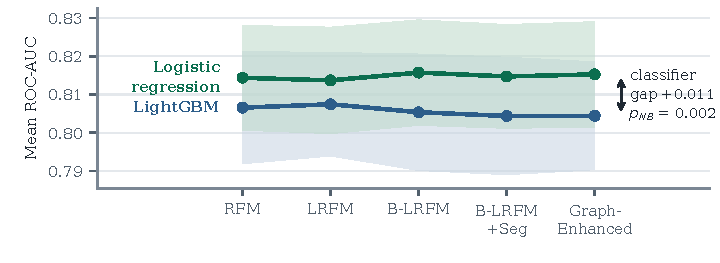
\includegraphics[width=\textwidth]{figures/fig_folds.pdf}
\caption{Mean ROC-AUC over 50 folds for each tier and classifier. Bands show
$\pm 1$ standard deviation of the fold scores, the spread a single split is drawn
from.}
\label{fig:folds}
\end{figure}

\subsection{The Result Does Not Depend on the Graph Degree}

A negative result about a graph may be a result about one particular graph. We
therefore rebuilt the graph, the communities and the fold-local features at
$k \in \{5, 10, 15, 20\}$ and reran the full repeated-CV protocol at each
setting. Table~\ref{tab:ksweep} reports the outcome.

\begin{table}[t]
\centering
\caption{Graph-Enhanced versus the RFM baseline as the graph degree varies.
LightGBM, $10 \times 5$ paired folds at every setting; the graph, the Louvain
communities and the fold-local features are rebuilt for each $k$.}
\label{tab:ksweep}
\setlength{\tabcolsep}{8pt}
\begin{tabular}{rrrrr}
\toprule
$k$ & Edges & Communities & $\Delta$ vs RFM & $p_{\mathrm{NB}}$ \\
\midrule
5 & 16{,}902 & 31 & $-0.0006$ & 0.880 \\
10 & 33{,}426 & 20 & $-0.0021$ & 0.590 \\
15 & 50{,}054 & 16 & $+0.0017$ & 0.666 \\
20 & 66{,}652 & 16 & $-0.0027$ & 0.500 \\
\bottomrule
\end{tabular}
\end{table}

Quadrupling the edge count and halving the number of communities changes the
graph substantially and the conclusion not at all: no setting reaches
significance, and the sign of the difference is not even stable, turning positive
at $k = 15$ and negative at the three others. A quantity whose sign depends on a
tuning parameter it should not depend on is behaving like noise, which is what
the $p$-values say directly.

\subsection{Attribution Is Not Contribution}

Global SHAP values \cite{lundberg2017shap} on the graph-enhanced model rank
recency first ($1.087$) and monetary value second ($0.560$), followed by
neighbour churn rate ($0.250$), interpurchase time ($0.224$) and community churn
rate ($0.215$). Read as an importance ranking, this appears to confirm that the
neighbourhood aggregates matter: two of the top five features are graph-derived.

They do not matter for discrimination: the tier without the six graph features
(B-LRFM+Seg, $0.8044$) and the tier with them (Graph-Enhanced, $0.8044$) are
indistinguishable. This ablation drops all six graph features at once and does
not isolate either aggregate. This is a matter of definition rather than a
contradiction.
SHAP attributes how a \emph{fitted} model distributes credit across the features
it was given, so a feature correlated with both the target and the rest of the
feature set absorbs attribution while adding nothing the others did not already
carry. Attribution rank answers ``what is this model using?''; only an ablation
answers ``would removing it cost anything?'', and here it answers no.

\subsection{Relation to the Segmentation Baseline}

Our starting point \cite{viannafilho2026rfm} segments customers on discrete 1--5
RFM scores in three dimensions; we predict churn in a nine-dimensional continuous
space. Silhouette scores are not comparable across feature spaces, so we make no
clustering-quality claim: the baseline reports $0.398$ at $k = 4$ on its own
scoring space, while K-means and Louvain on our space reach $0.219$ and
$-0.050$. The relation between the two works is scope extension, not
improvement. The communities remain usable for prioritisation: ranked by churn
probability times monetary value, they separate a high-value at-risk group
($327$ customers, $82\%$ churn) from a high-value loyal one ($418$ customers,
$24\%$ churn), a descriptive output only, since the data contain no campaign
responses.

\section{Discussion}
\label{sec:disc}

\subsection{Effect Sizes Below the Noise Floor}

Two independent sources of variation are the same size as the effects the
pipeline was built to detect. The fold partition contributes roughly $0.003$
ROC-AUC, as the sign reversal above shows. Library versions contribute as much:
re-running the auxiliary improvement pipeline under newer libraries moved its best
configuration by $-0.0033$ ROC-AUC and the Leiden community count from $20$ to
$21$. We therefore treat differences below roughly $0.005$ ROC-AUC on this dataset
as uninformative, and suggest that comparisons here either report a
variance-corrected test or refrain from ranking configurations inside that band.

\subsection{Why the Contagion Hypothesis Might Still Hold}
\label{sec:contagion}

Our result is a failure to reject a null on one dataset with one graph
construction, not a demonstration that behavioural peer effects are absent. The
most likely explanation is that we built the wrong graph: its edges encode
proximity in a feature space derived from the same purchase history that already
feeds the classifier, so the neighbour churn rate is plausibly a smoothed
restatement of what the model has rather than new information. This reading is
consistent with where the feature does work. The telecommunications and social
graph results cited in Sect.~2 are built on recorded interaction (who called
whom, who plays with whom), not on similarity computed from the model's own
inputs \cite{kostic2020socialnetwork,lee2025tempodegraphnet}.

Churn itself also differs between the two settings. In telecommunications it is
the cancellation of a service contract, and peers have a way to influence each
other: people who call each other benefit from staying on the same network, and
a subscriber's churn risk has been linked to the number of contacts who have
already left \cite{kostic2020socialnetwork}. In non-contractual retail nobody
cancels. Churn is inferred from a gap in purchases, and two customers who buy
alike need not know each other. A similarity graph therefore connects customers who resemble each
other, not customers who influence each other, and its neighbourhood churn rate
can at most summarise what similar customers did, which the classifier already
sees in the features. A retail graph built from interactions absent from the
feature matrix, such as shared baskets, referral or household links, would be a
different test, and is the experiment we would run next.
Two weaker readings also fit: a three-month inactivity label on a majority-churn
base may be too coarse for neighbourhood effects to surface, and with all tiers
near $0.81$ ROC-AUC the binding constraint may be the representation rather than
the model class.

\section{Threats to Validity}

All results come from one retailer over two years, so we make no claim about
other sectors or horizons, and the effect-size floor we report holds only for
this dataset and sample size. The degree sweep rules out an artefact of $k$, but
every graph we tried is a $k$-NN graph on the same features, and graphs built
from interactions remain untested (Sect.~\ref{sec:contagion}). Two parts of the
original study design, a country-of-origin encoding and spectral clustering, were
never implemented and play no role in the results. Because churners are the
majority class, \mbox{PR-AUC} loses its usual meaning here, and no conclusion
rests on it alone.

Our literature search was targeted rather than systematic. The studies of
neighbourhood churn that we found (Sect.~2) use interaction graphs, but we make
no priority claim. Finally, the expected retention value ranks customers by
a model output, not by observed campaign response, so its practical value is
untested.

\section{Conclusion}

We built the pipeline the behavioural-peer-effect hypothesis calls for and
evaluated it under fold-local recomputation of the label-derived features and
repeated cross-validation with a corrected test. The hypothesis is not supported
on this dataset at any graph degree tested. The significant differences we found
are between classifiers and say nothing about the graph features.

The methodological point generalises further than the negative result. An
evaluation that reports one cross-validated number per configuration cannot
distinguish a $0.003$ ROC-AUC difference from the partition that produced it. The
controls used here are inexpensive (ten repetitions of five-fold
cross-validation on $5{,}038$ customers take minutes), and we would argue they
belong in the default protocol rather than in an appendix.

\subsubsection{Reproducibility.}
Code, per-fold scores, significance summaries and raw run logs are available at
\url{https://github.com/VoDucNhatku/graph-neighbourhood-churn-fisat2026}, tagged
\texttt{v1.1}. Library versions are pinned to the environment that
produced every reported number, and Fig.~\ref{fig:folds} and
Table~\ref{tab:cross} are computed from the committed per-fold scores. The full
pipeline runs in under ten minutes on a laptop with no GPU.

\begin{credits}
\subsubsection{\ackname}
The authors used a large language model (Claude, Anthropic) to draft and revise
the manuscript, write parts of the evaluation and figure code, and cross-check
numbers against the result files. All numbers were verified against the archived
runs, and the authors take full responsibility for the content.

\subsubsection{\discintname}
The authors have no competing interests to declare that are relevant to the
content of this article.
\end{credits}

\bibliographystyle{splncs04}
\bibliography{refs}

\end{document}
